
\section{Cut-running and fractal tesseract}\label{sec:cut-running-fractal-tesseract}

\subsection{Null presentation}\label{subsec:null-presentation}
\begin{definition}[Null symmetry]
The A\(\Omega\)D form of the AFC Null potential is
\begin{equation}
\Null\equiv \infD,
\label{eq:null-axiom}
\end{equation}
where \(\infD\) names unresolved possible distinction. Null names symmetric closure under which branch selection is presented.
\end{definition}

The Null presentation preserves the same syntax as the local cut-running form:
\begin{equation}
\Null\equiv\infty
\qquad
\Null\to\Null\to\Null\equiv\Null.
\label{eq:null-presentation}
\end{equation}

\subsection{Local cut-running form}\label{subsec:local-cut-running-form}
\begin{definition}[Cut operator]
The A\(\Omega\)D cut operator sends a retained occurrence into simultaneous identity and cut-running:
\begin{equation}
x\mapsto x\succ x=x.
\label{eq:cut-running-form}
\end{equation}
The symbol \(\succ\) names asymmetric cut-running. The expression records that the same \(x\) is held in identity while also presenting a running cut relation.
\end{definition}

\paragraph{Stokes identity as temporal dynamics.}
The cut operator presents the Stokes identity as temporal dynamics. A null bounds its unspooled infinity of nulls and returns to null. This completed return is the monon cycle:
\begin{equation}
\mathrm{monon}(x)=\operatorname{cycle}(x\succ x=x).
\label{eq:monon-cycle}
\end{equation}
The monon is the first completed beat of the cut operator. It is the primitive completion marker of A\(\Omega\)D return dynamics.

\paragraph{Simultaneous presentation.}
The null potential is symmetric in totality. The cut operator unspools that symmetry into temporal asymmetry. Motion is the rebalancing of the unspooled asymmetry toward symmetric closure. The rebalancing has no terminal global end because the null remains simultaneously symmetric while cut-running continues. Local completion is the monon beat: null-to-unspooled-boundary-to-null return.

\paragraph{Inheritance.}
Each occurrence of \(x\) inherits the same primitive presentation:
\[
x\mapsto (x\succ x=x).
\]
Thus
\[
x
\Rightarrow (x\succ x=x)
\Rightarrow ((x\succ x=x)\succ(x\succ x=x)=(x\succ x=x))
\Rightarrow \cdots.
\]
The cut begets a cut because every presented occurrence can present the same simultaneous identity and running relation.

\subsection{Branch / hinge / branch}\label{subsec:branch-hinge-branch}
\begin{definition}[Branch / hinge / branch]
A retained cut-running presentation distinguishes branch, hinge, and branch. The branches are the two retained occurrences exposed by the cut-running relation. The hinge is the middle occurrence through which return, dwell, pinning, reseating, or closure can occur.
\end{definition}

\subsubsection{Hinge triad}\label{subsec:hinge-triad}
\begin{definition}[Hinge triad]
The branch/hinge/branch support is the hinge triad
\[
\mathsf H_3=(x^-,\mu,x^+).
\]
Here \(x^-\) is the past branch, \(\mu\) is the hinge / dwell / pivot, and \(x^+\) is the future branch. Its local ternary support is
\[
\{-1,0,+1\}.
\]
\end{definition}

\subsubsection{Crown}\label{subsec:crown}
Use the direct temporal terms
\[
x^- = \text{past},
\qquad
x^0 = \text{present},
\qquad
x^+ = \text{future}.
\]
The temporal dynamic is
\[
x^-\to x^0\to x^+.
\]
The field holds past, present, and future in symmetric totality. The cut crowns the present:
\[
\operatorname{Crown}(x)=x^0.
\]
Temporal dynamics is the asymmetric unspooling of this symmetric totality.

\paragraph{Retained ternary support.}
When branch/hinge/branch is retained locally, its coarse support is
\[
\{-1,0,+1\}.
\]
The value \(0\) is hinge, dwell, or pivot. The values \(-1\) and \(+1\) are branch orientations. For \(k\) unconstrained retained positions, the retained base-3 capacity is
\[
C_3(k)=\log_3(3^k)=k.
\]
This capacity is carried by duon current and by entropic duon current when unresolved return burden is retained.

\subsection{Fractal tesseract}\label{subsec:fractal-tesseract}
\subsubsection{Recursive support}\label{subsec:fractal-recursive-support}
The fractal tesseract is the self-similar branch/hinge/branch topology of recursive cut-running. Recursive cut-running preserves branch, hinge, and branch across nested presentations. Each retained occurrence inherits \(x\succ x=x\) and can run the cut again. The result is recursive incidence, return, and enclosure.

\subsubsection{Jitter}\label{subsec:fractal-jitter}
Jitter is unresolved successor movement inside the fractal tesseract topology. Before a carried current has seated, the next branch/hinge/branch continuation can remain unsettled. Jitter is the local motion of successor possibility before return stabilizes.

\subsubsection{Four-edge x witness}\label{subsec:four-edge-x-witness}
A retained \(x\)-occurrence in the finite \(\Qfour\) witness is a vertex
\[
\epsilon=(\epsilon_1,\epsilon_2,\epsilon_3,\epsilon_4)\in\{0,1\}^4.
\]
The four active dion positions supply the four tesseract-edge directions:
\[
\epsilon \leftrightarrow \epsilon\oplus e_i,
\qquad i=1,2,3,4.
\]
Thus every retained \(x\)-vertex in the local witness has
\[
\deg_{\Qfour}(\epsilon)=4.
\]
The monon hinge \(\mu\) remains the ternary fibre over that four-edge support.

\begin{figure}[H]
\centering
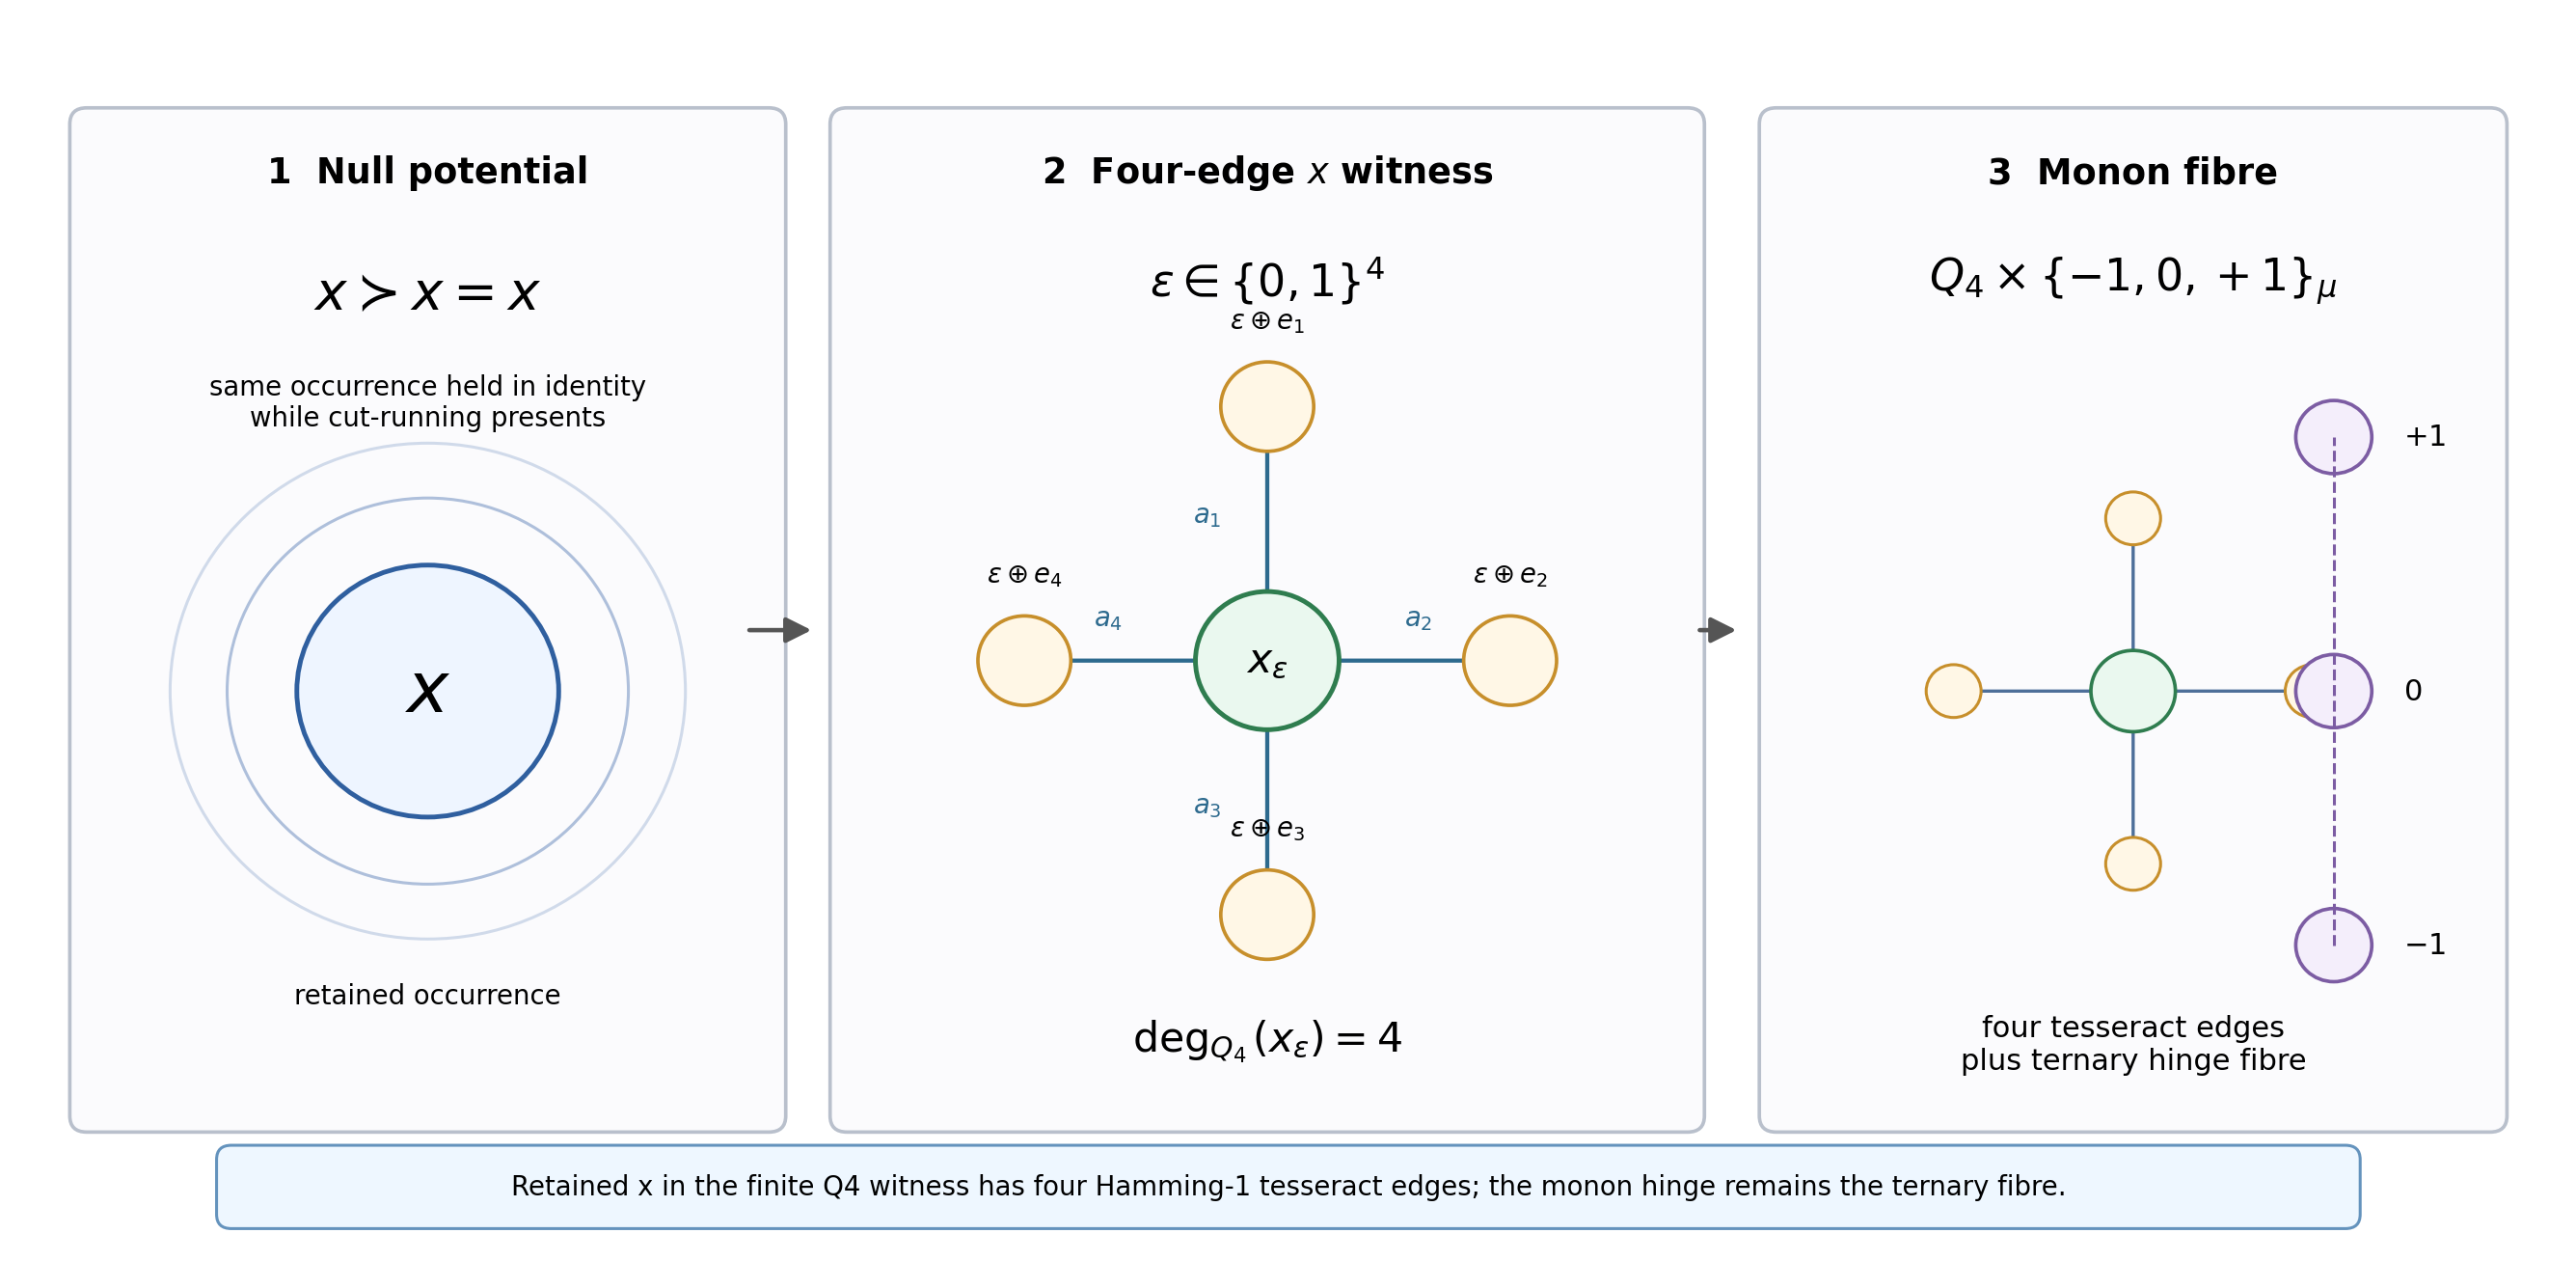
\includegraphics[width=0.96\linewidth]{figures_jpg/null_four_edge_x_witness.png}
\caption{Null-to-tesseract four-edge witness.}
\label{fig:null-four-edge-x-witness}
\end{figure}

\subsubsection{Finite Q4 witness}\label{subsec:finite-q4-witness}
A finite \(\Qfour\) chart is a local witness of the fractal tesseract topology. A resolved duon has four active dion positions and one carried monon hinge. Partial unspooling of the four active positions gives \(\{0,1\}^4\). Hamming-1 adjacency gives \(\Qfour\). The middle hinge remains the ternary fibre.

\begin{figure}[H]
\centering
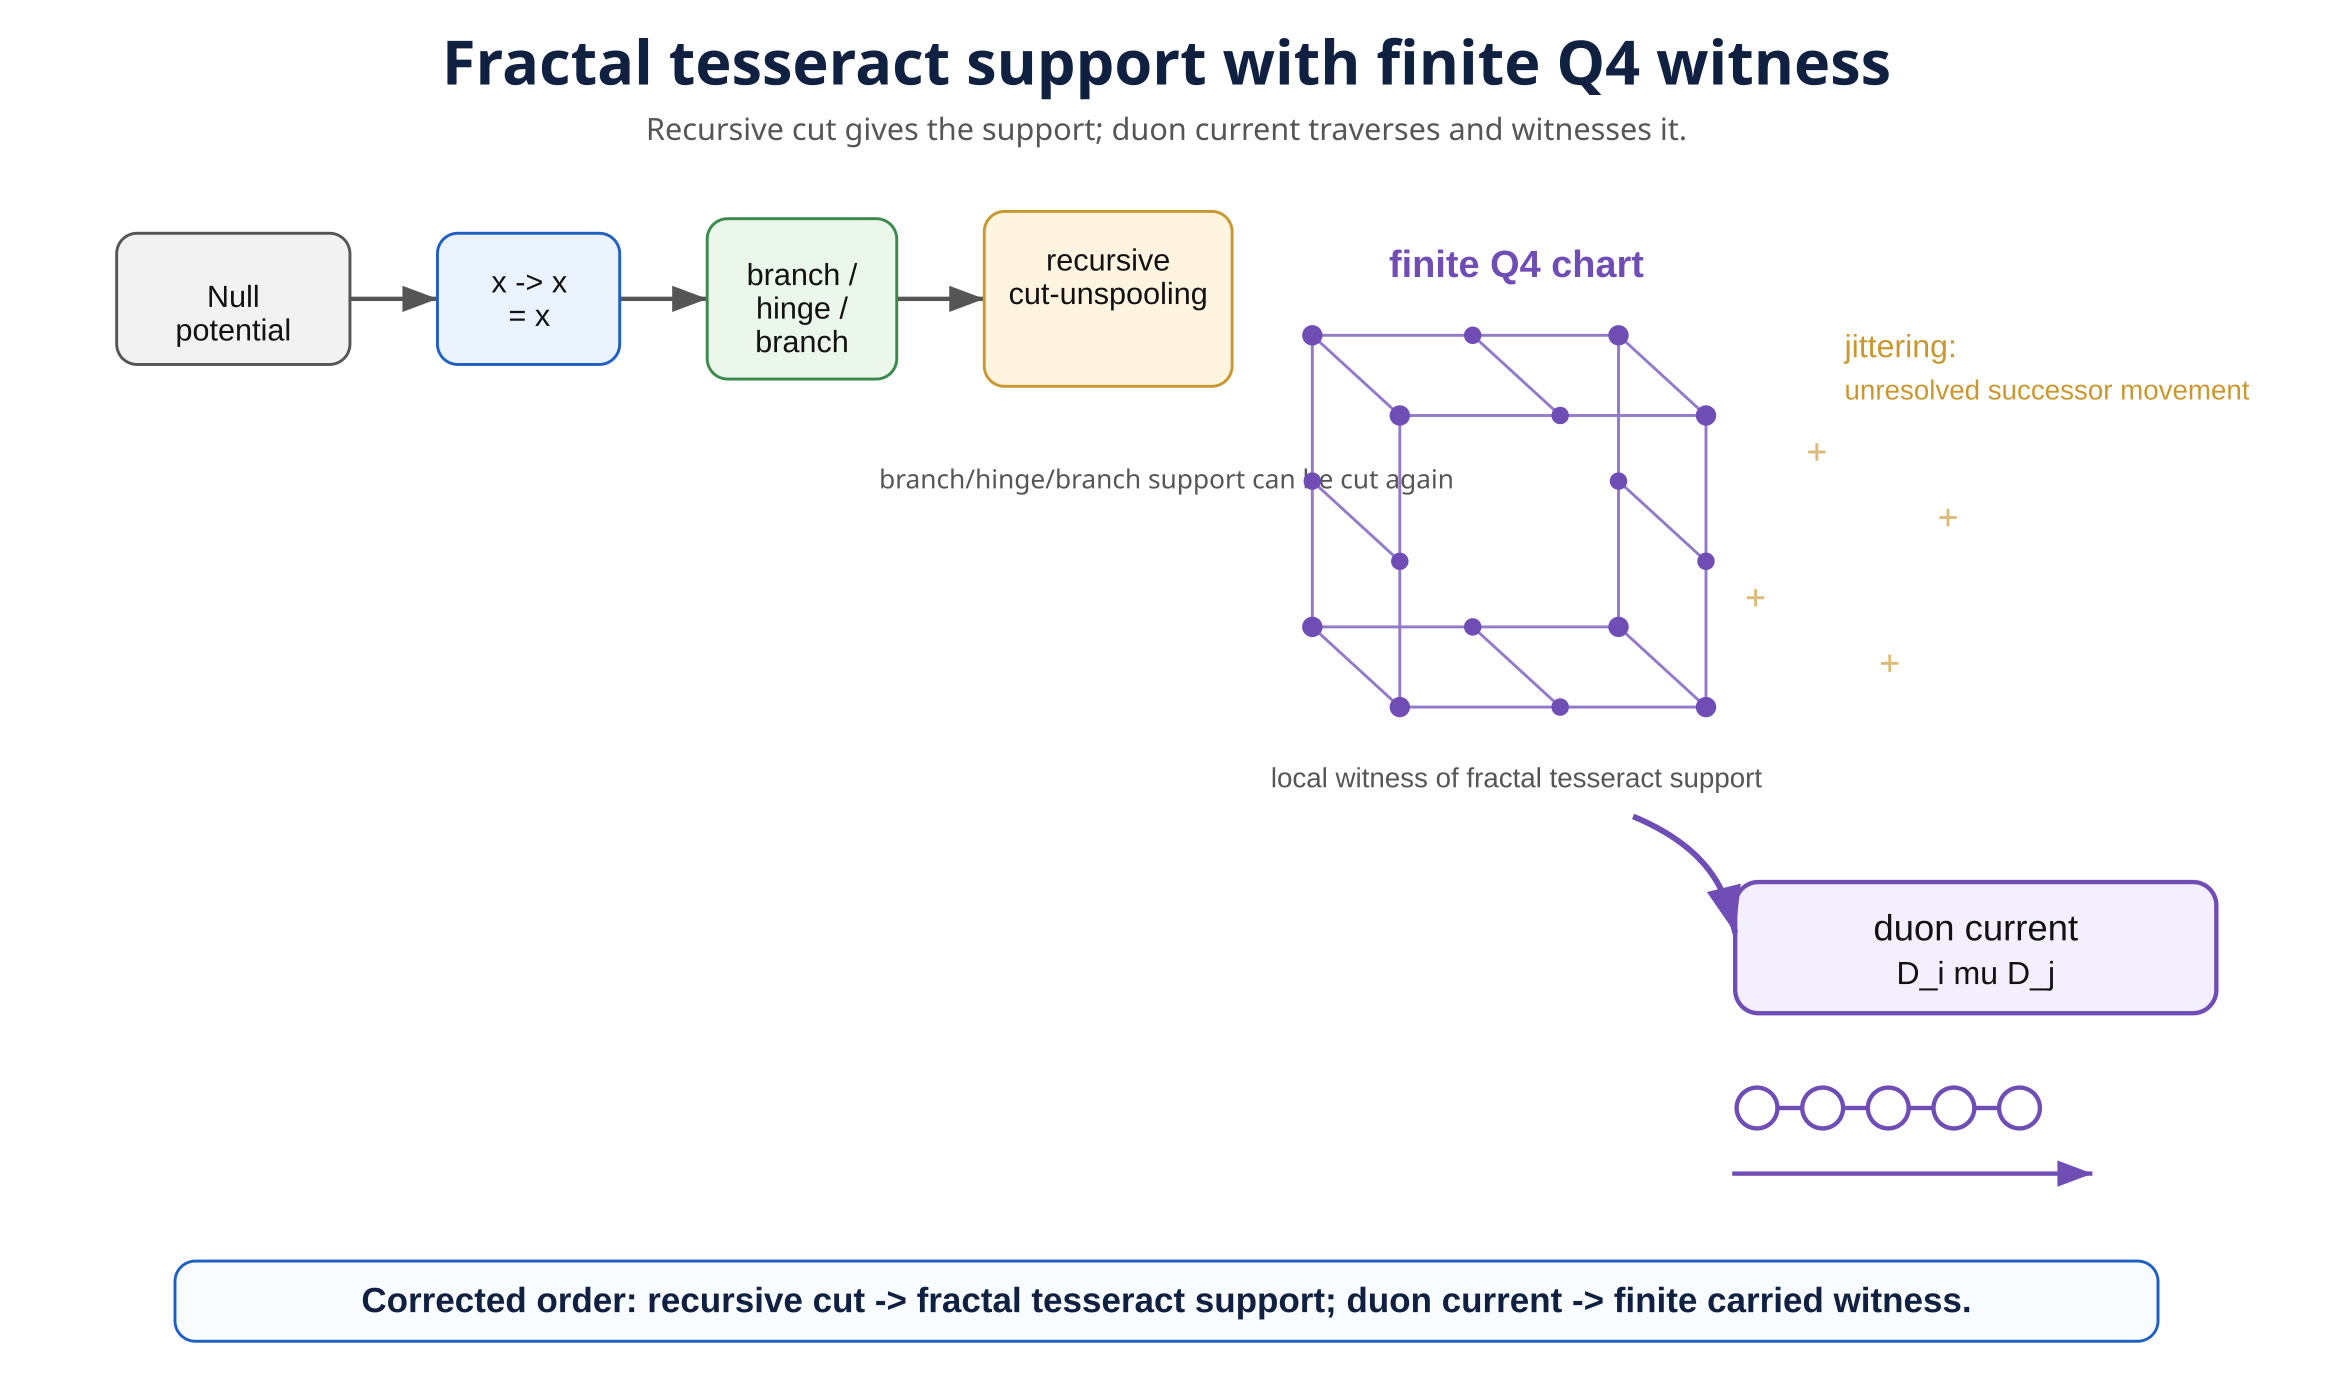
\includegraphics[width=0.96\linewidth]{figures_jpg/fractal_tesseract_q4_witness.jpg}
\caption{Fractal tesseract support with finite \(\Qfour\) witness.}
\label{fig:v39-fractal-tesseract-q4-witness}
\end{figure}



\subsubsection{Hamming--1 graph and ternary kernel}\label{subsec:q4-hamming-ternary-kernel}
\paragraph{Setup.}
The finite tesseract support is the Hamming--1 graph
\[
V(Q_4)=\{0,1\}^4,
\qquad
E(Q_4)=\{(x,y):d_H(x,y)=1\},
\]
where
\[
d_H(x,y)=\#\{k:x_k\ne y_k\}.
\]

\paragraph{Definition.}
A local tick/click state on an oriented edge carries the ternary fibre
\[
\sigma_t(e)\in\{-1,0,+1\},
\]
with \(+1\) out-bound, \(0\) hinge / dwell, and \(-1\) return-bound.

\paragraph{Choice.}
A max-capacity-3 Markov kernel on the declared scope is
\[
P_B((e',\sigma')\mid(e,\sigma))\ge0,
\qquad
\sum_{(e',\sigma')}P_B((e',\sigma')\mid(e,\sigma))=1,
\]
with
\[
P_B((e',\sigma')\mid(e,\sigma))=0
\quad\text{outside admissible Hamming--1 continuations},
\qquad
\sigma'\in\{-1,0,+1\}.
\]
The isotropic choice is
\[
P_B^{\mathrm{iso}}((e',\sigma')\mid(e,\sigma))=
\frac{1}{N_B(e,\sigma)}
\]
over admissible successors. The anisotropic choice is
\[
P_B^{\mathrm{ani}}((e',\sigma')\mid(e,\sigma))=
\frac{w_B(e',\sigma')}
{\sum_{(a,\vartheta)\in\operatorname{Adm}_B(e,\sigma)}w_B(a,\vartheta)},
\]
where the weights may depend on \(\Delta\chi^{\mathrm{lag}}_{e'}(B)\),
\(i_{e'}(B)\), and \(R^{\mathrm{asym}}_{e'}(B)\).


\paragraph{Four-edge implementation.}
At a vertex of \(Q_4\), the current oriented edge may be treated as the ancestor edge of the local tick/click step.  The four Hamming--1 incident edge slots consist of that retained ancestor slot together with up to three successor slots.  The successor pool carries the ternary fibre \(\{-1,0,+1\}\): return branch, hinge/dwell, and outbound branch.  The isotropic kernel assigns equal weight to admissible successor states; the anisotropic kernel reweights the same admissible states by the declared boundary data.  When the hinge state reaches capacity on the declared scope, same-resolution dwell is unavailable and the continuation is branch/hinge/branch through the remaining admitted branch states.

The hinge-continuation family is
\begin{equation}
\operatorname{Adm}^{0}_{B}(e,\sigma)
=
\{(e',0)\in\operatorname{Adm}_{B}(e,\sigma)\}.
\label{eq:hinge-admissible-family}
\end{equation}
Hinge saturation is
\begin{equation}
\operatorname{Adm}^{0}_{B}(e,\sigma)=\varnothing,
\label{eq:hinge-saturation}
\end{equation}
or, in the weighted kernel,
\begin{equation}
\sum_{(e',0)\in\operatorname{Adm}_{B}(e,\sigma)}w_B(e',0)=0.
\label{eq:hinge-saturation-weighted}
\end{equation}
When \(\operatorname{Adm}^{0}_{B}(e,\sigma)=\varnothing\), the continuation is branch-oriented,
\begin{equation}
\sigma'\in\{-1,+1\},
\label{eq:hinge-saturation-branch-continuation}
\end{equation}
until reseating, shedding, pass-through, or coordinate lift. Jitter is unresolved successor motion before seating; hinge saturation removes same-resolution dwell and forces branch-oriented continuation.

\aodliteraturenote{Hypercube/Hamming--1 support: Weisstein~\cite{weissteinHypercubeGraph}.}
\aodliteraturenote{Adjacency-walk counts: MIT OCW~\cite{mitAdjacencyWalks}, Duncan~\cite{duncanAdjacencyWalks}.}
\aodliteraturenote{Graph random walks and Markov kernels: Wisconsin~\cite{wisconsinRandomWalks}, Norris~\cite{norrisMarkov}, Levin--Peres--Wilmer~\cite{levinPeresWilmer}, Lawler--Limic~\cite{lawlerLimic}.}
\aodliteraturenote{Dyck/Catalan paths: Stanley~\cite{stanleyCatalan}, Flajolet--Sedgewick~\cite{flajoletSedgewick}.}

\aodremark{The \(Q_4\) chart is a finite Hamming--1 graph. The kernel supplies admissible tick/click histories; it does not replace the scoped flux calculation.}


\paragraph{Definition.}
A tesseract-admissible boundary is a retained shell cut through the finite Hamming--1 support:
\begin{equation}
\partial_TF\subseteq E(\Qfour)\times\{-1,0,+1\}.
\label{eq:tesseract-admissible-boundary}
\end{equation}
The boundary/window scope is
\begin{equation}
B=(\partial_TF,\omega).
\label{eq:tesseract-boundary-window}
\end{equation}
A calculation may record values computed on \(B\). The boundary is fixed by the retained tesseract-admissible shell cut.

\aodprovenance{\eqnref{eq:null-presentation}, \eqnref{eq:cut-running-form}, \eqnref{eq:monon-cycle}, \appref{app:curling-curls}.}